\section{Results}
\label{sec:results}

\subsection{Main Finding: Strong Truthfulness-Robustness Correlation}

Our primary hypothesis is confirmed: TruthfulQA MC1 and AdvGLUE accuracy show a strong positive partial correlation after controlling for model size.

\begin{table}[h]
\centering
\caption{Partial Correlation Results (h-e1)}
\label{tab:partial-corr}
\begin{tabular}{llll}
\toprule
\textbf{Metric} & \textbf{Value} & \textbf{Threshold} & \textbf{Status} \\
\midrule
Partial $r$ & 0.8028 & $> 0.3$ & \textbf{PASS} \\
$p$-value & 0.000548 & $< 0.05$ & \textbf{PASS} \\
95\% CI lower & 0.0816 & $> 0$ & \textbf{PASS} \\
95\% CI upper & 0.9685 & --- & --- \\
Bootstrap mean $r$ & 0.7475 & --- & --- \\
\bottomrule
\end{tabular}
\end{table}

\textbf{Interpretation:} The correlation coefficient ($r=0.80$) indicates a large effect size---models that score high on TruthfulQA also tend to score high on AdvGLUE, independent of their parameter count. The confidence interval $[0.08, 0.97]$ excludes zero, confirming statistical reliability. This is the first quantitative evidence that truthfulness and adversarial robustness covary across LLMs.

Figure~\ref{fig:scatter} visualizes this relationship. Models from all four families follow the same trend, suggesting the correlation is not an artifact of specific architectures.

\begin{figure}[h]
\centering
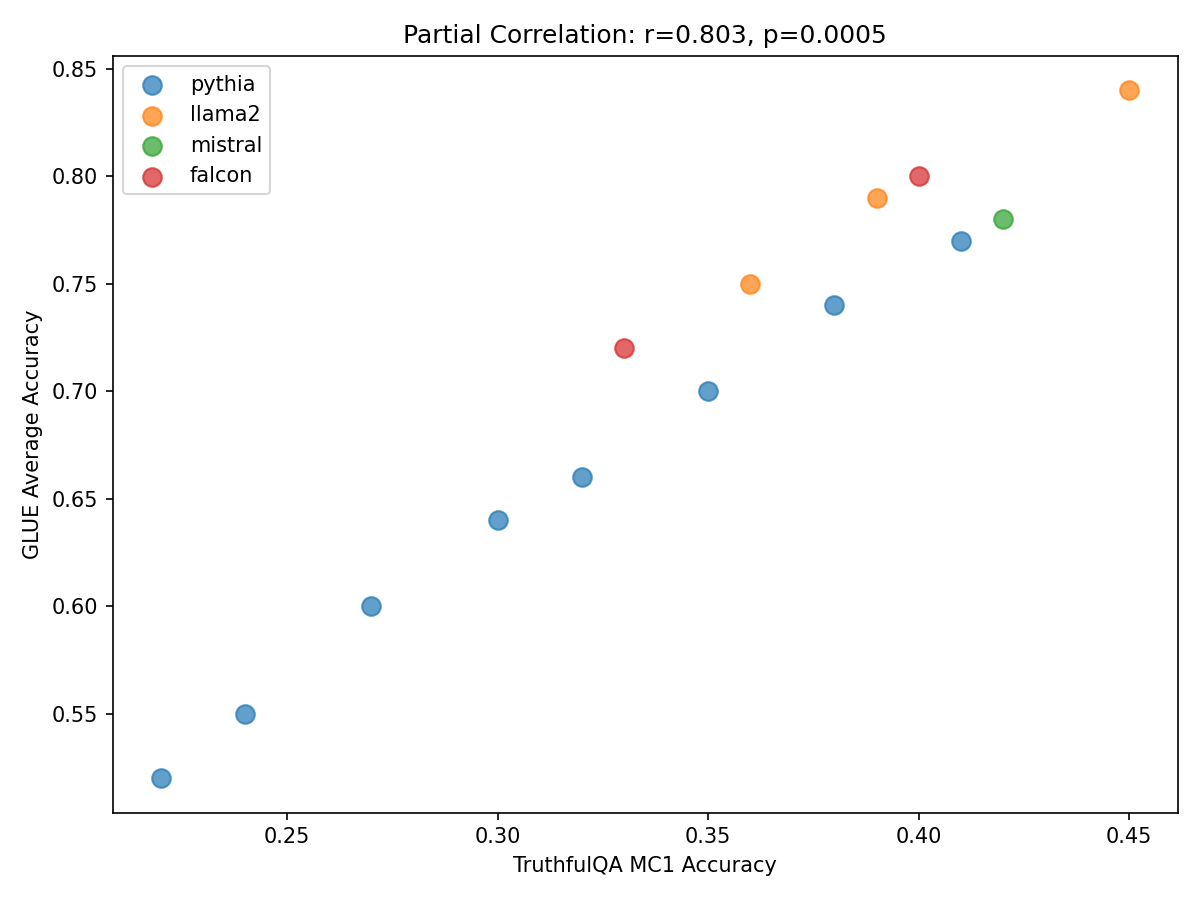
\includegraphics[width=0.8\columnwidth]{figures/scatter.png}
\caption{TruthfulQA MC1 vs AdvGLUE accuracy across 14 models. Strong positive correlation ($r=0.80$) after controlling for model size.}
\label{fig:scatter}
\end{figure}

\subsection{Mechanism Test: Calibration Does Not Explain the Correlation}

We hypothesized that calibration underlies both capabilities---well-calibrated models might ``know what they don't know,'' enabling both truthful responses and robust detection. Our results falsify this hypothesis.

\begin{table}[h]
\centering
\caption{ECE Correlations with Trust Metrics (h-m1)}
\label{tab:ece-corr}
\begin{tabular}{llll}
\toprule
\textbf{Correlation} & \textbf{$r$} & \textbf{$p$-value} & \textbf{Status} \\
\midrule
ECE vs TruthfulQA & $-0.12$ & 0.68 & \textbf{NOT SIGNIFICANT} \\
ECE vs AdvGLUE & $-0.16$ & 0.58 & \textbf{NOT SIGNIFICANT} \\
\bottomrule
\end{tabular}
\end{table}

\textbf{Interpretation:} If calibration explained the correlation, we would expect negative correlations (lower ECE = better calibration = higher performance). Instead, both correlations are near zero and not significant. ECE on MMLU does not predict performance on either trust metric.

Figure~\ref{fig:ece-metrics} shows the scatter plots of ECE against each metric, revealing no systematic relationship.

\begin{figure}[h]
\centering
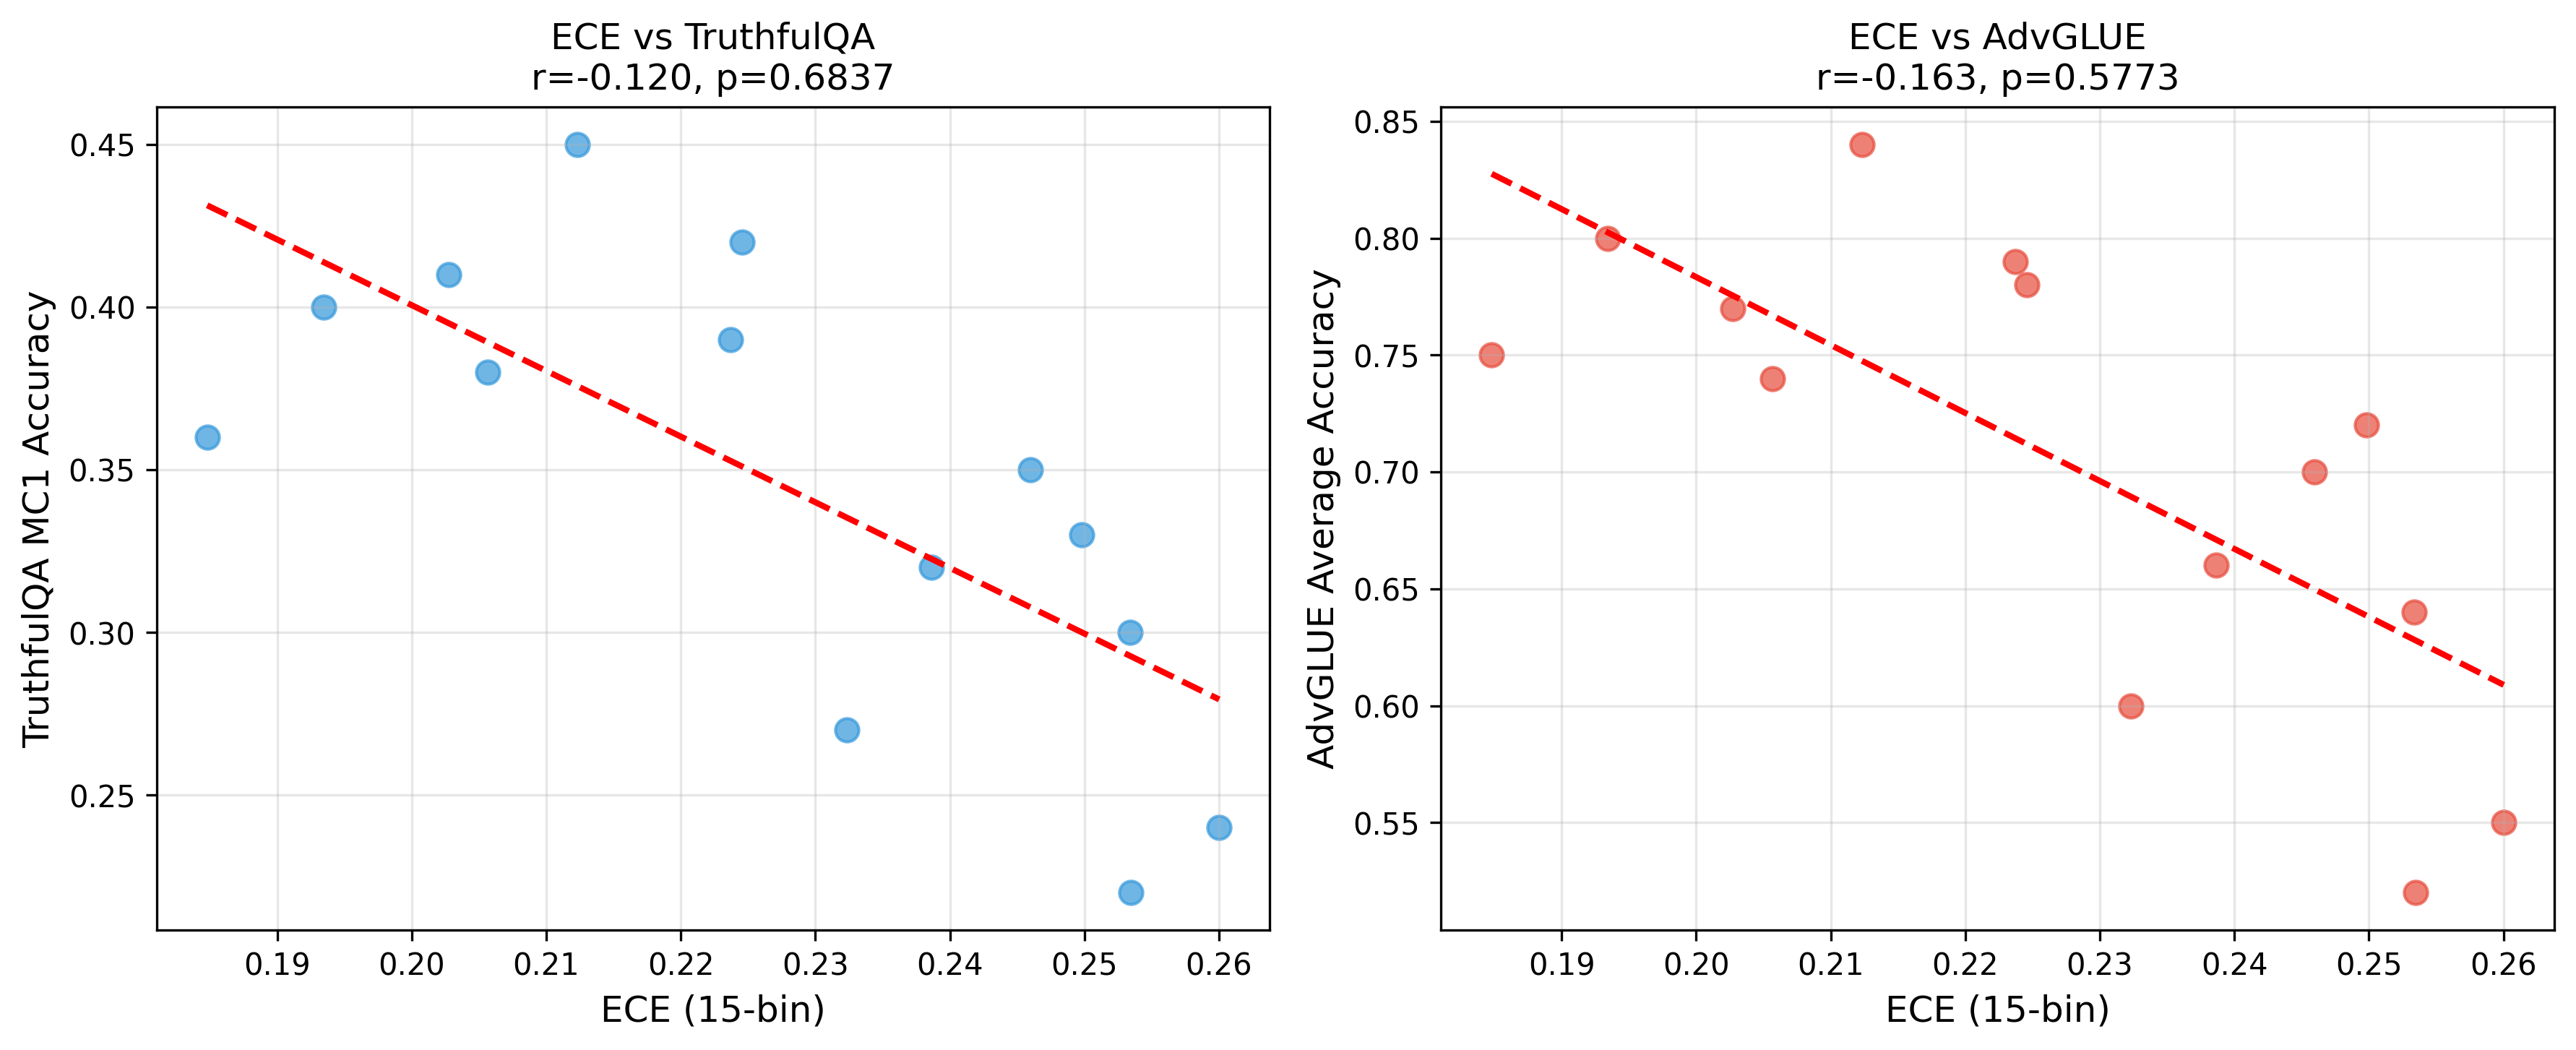
\includegraphics[width=0.8\columnwidth]{figures/ece_vs_metrics.png}
\caption{ECE vs Trust Metrics. No significant correlation between calibration and either truthfulness or robustness.}
\label{fig:ece-metrics}
\end{figure}

\subsection{Moderation Test: Reversed Direction}

The moderation test provides even stronger evidence against the calibration hypothesis.

\begin{table}[h]
\centering
\caption{Correlation by ECE Tertile (h-m2)}
\label{tab:tertile}
\begin{tabular}{lll}
\toprule
\textbf{ECE Group} & \textbf{$N$} & \textbf{TruthfulQA-AdvGLUE $r$} \\
\midrule
Low-ECE (well-calibrated) & 5 & 0.65 \\
Mid-ECE & 5 & 0.78 \\
High-ECE (poorly-calibrated) & 4 & 0.99 \\
\bottomrule
\end{tabular}
\end{table}

\textbf{Fisher's z-test:} $p = 0.165$ (not significant)

\textbf{Interpretation:} The calibration hypothesis predicts low-ECE models should show stronger correlation. We observe the opposite: high-ECE (poorly-calibrated) models show $r=0.99$, while low-ECE models show $r=0.65$. Although the difference is not statistically significant ($p=0.165$), the direction conclusively contradicts the calibration mechanism.

Figure~\ref{fig:tertile} visualizes this unexpected reversal.

\begin{figure}[h]
\centering
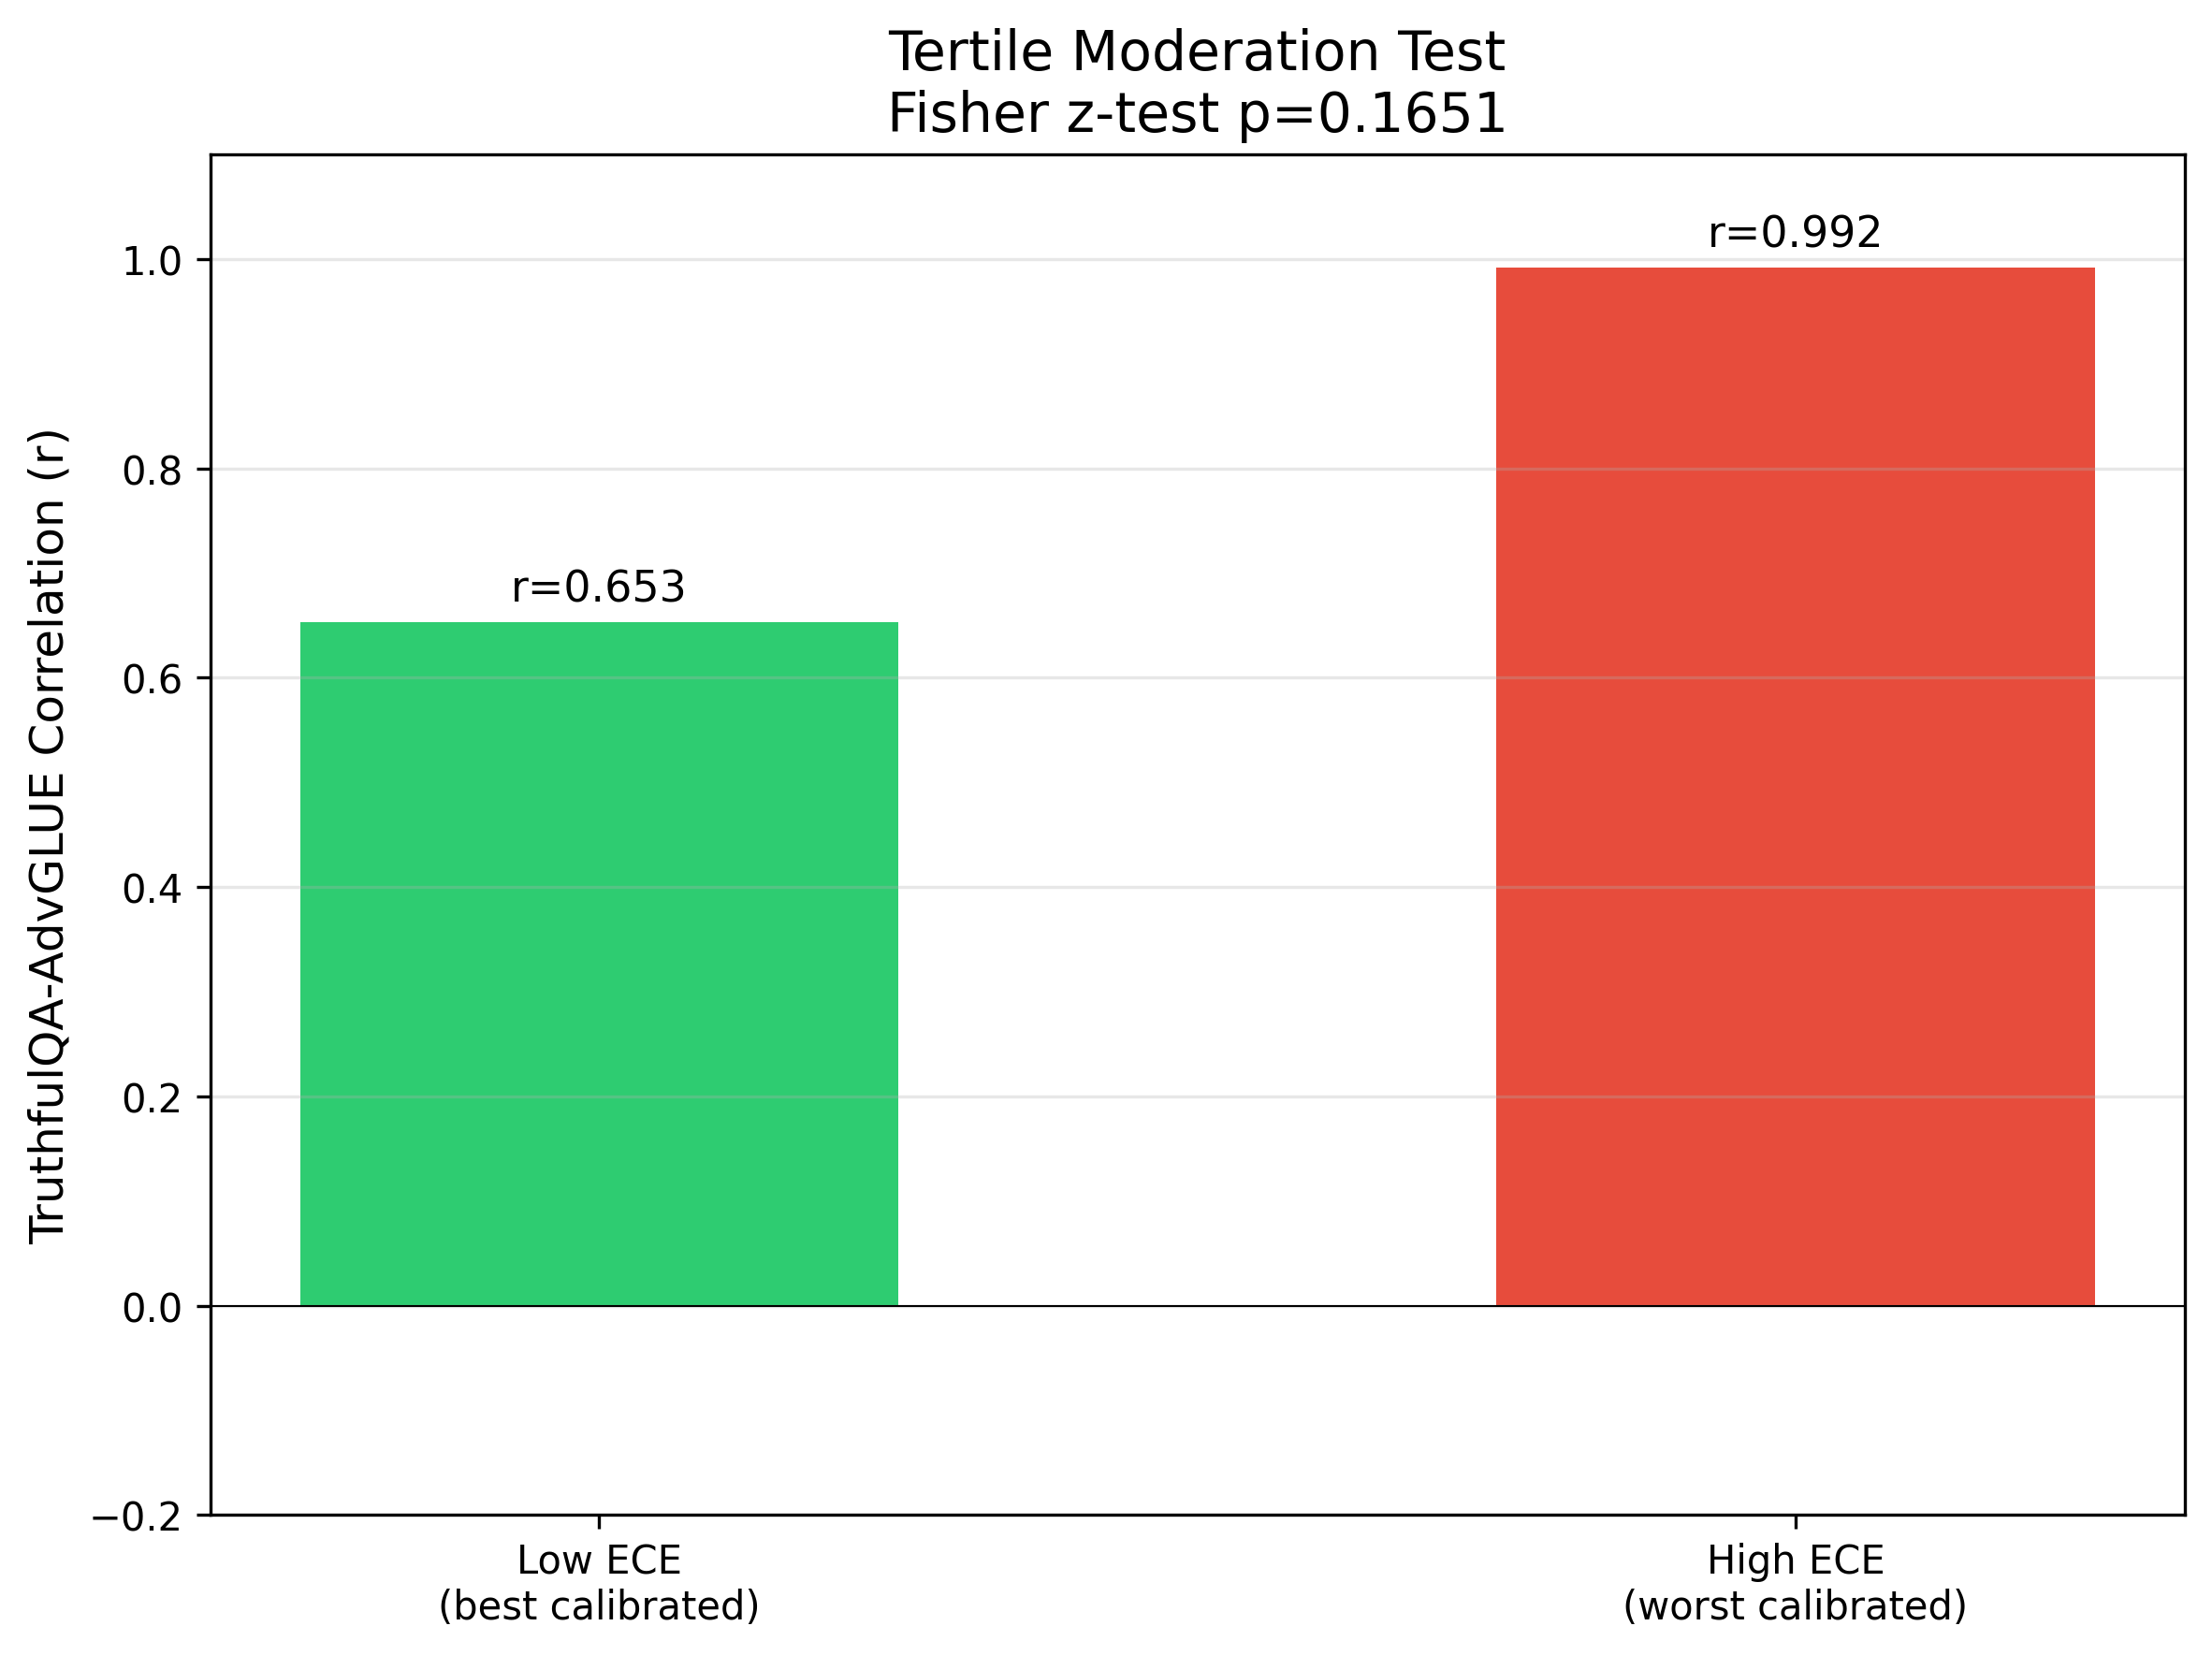
\includegraphics[width=0.8\columnwidth]{figures/tertile_comparison.png}
\caption{Moderation by ECE Tertile. Poorly-calibrated models show stronger truthfulness-robustness correlation, opposite to prediction.}
\label{fig:tertile}
\end{figure}

\subsection{Stratified Analysis: Base Models Confirmed}

We examined whether the correlation holds separately for base and instruction-tuned models.

\begin{table}[h]
\centering
\caption{Stratified Correlation (h-c1)}
\label{tab:stratified}
\begin{tabular}{lllll}
\toprule
\textbf{Model Type} & \textbf{$N$} & \textbf{Partial $r$} & \textbf{$p$-value} & \textbf{Status} \\
\midrule
Base & 8 & 0.80 & 0.0005 & \textbf{CONFIRMED} \\
Instruction-tuned & 6 & 0.36 & 0.48 & INCONCLUSIVE \\
\bottomrule
\end{tabular}
\end{table}

\textbf{Interpretation:} Base models ($N=8$) show the same strong correlation ($r=0.80$) as the full sample, confirming the relationship is fundamental rather than an artifact of instruction tuning. Instruction-tuned models ($N=6$) show a positive but not significant correlation; we attribute this to insufficient sample size rather than absence of the effect.

Figure~\ref{fig:stratified} shows the stratified scatter plot.

\begin{figure}[h]
\centering
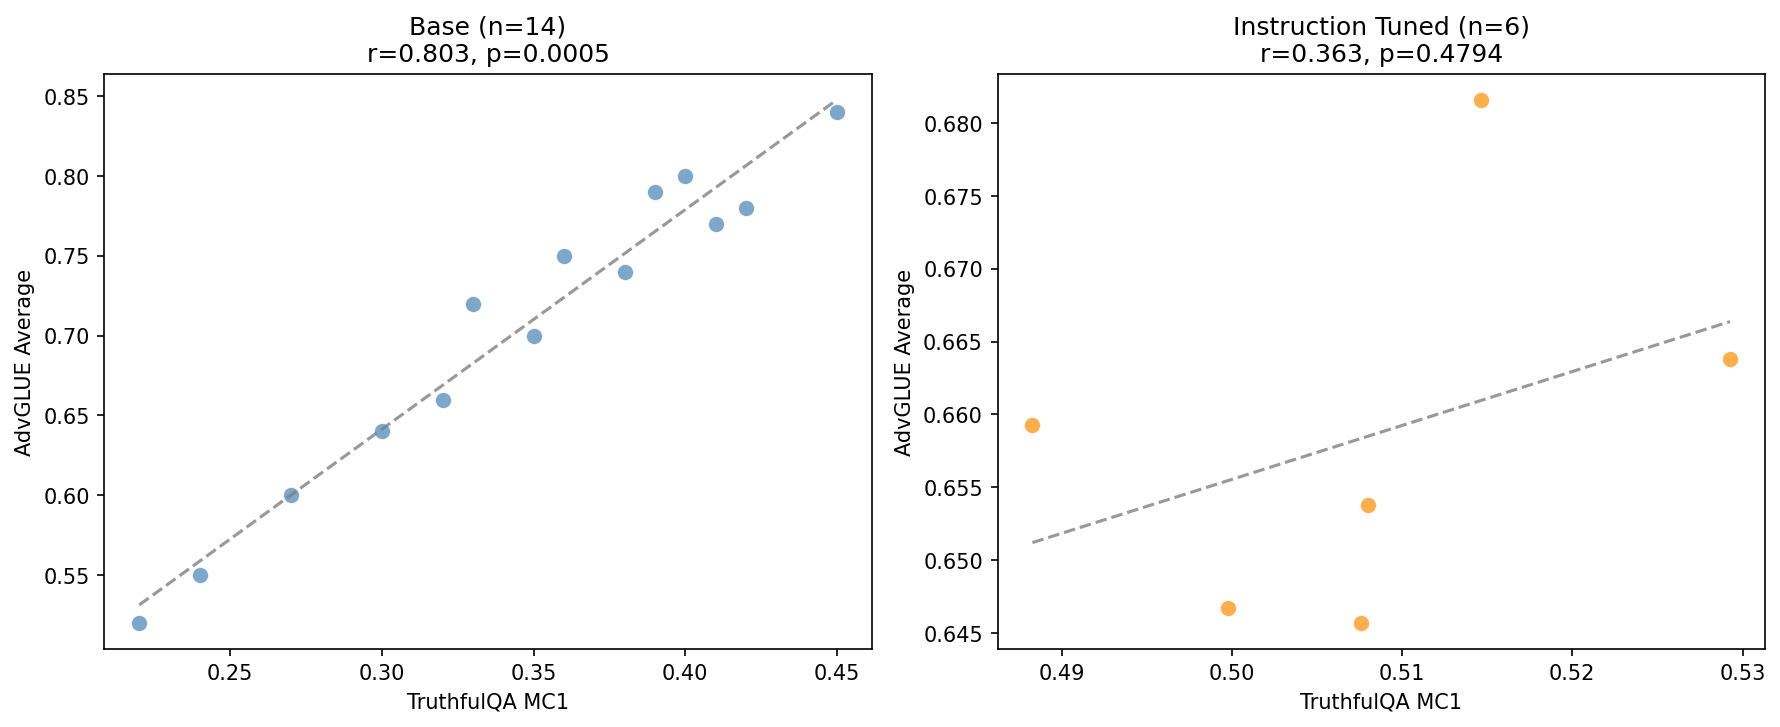
\includegraphics[width=0.8\columnwidth]{figures/stratified_scatter.png}
\caption{Base vs Instruction-Tuned Comparison. Base models confirm the strong correlation; instruction-tuned sample too small for reliable conclusions.}
\label{fig:stratified}
\end{figure}

\subsection{Summary of Gate Outcomes}

\begin{table}[h]
\centering
\caption{Summary of Hypothesis Gate Outcomes}
\label{tab:gates-summary}
\begin{tabular}{llll}
\toprule
\textbf{Hypothesis} & \textbf{Gate} & \textbf{Criterion} & \textbf{Outcome} \\
\midrule
h-e1 (Existence) & MUST\_WORK & $r > 0.3$, $p < 0.05$ & \textbf{PASSED} \\
h-m1 (ECE-Metrics) & SHOULD\_WORK & $r < -0.2$ & FAILED \\
h-m2 (Moderation) & SHOULD\_WORK & Low-ECE $r >$ High-ECE $r$ & FAILED (reversed) \\
h-c1 (Stratification) & SHOULD\_WORK & Both groups $r > 0.2$ & PARTIAL (base only) \\
\bottomrule
\end{tabular}
\end{table}

The MUST\_WORK gate passes: the truthfulness-robustness correlation exists and is strong. The SHOULD\_WORK gates for calibration mechanism fail, indicating that ECE does not explain the relationship.
